%%%%%%%%%%%%%%%%%%%%%%%%%%%%%%%%%%%%%%%%%%%%%%%%%%%%%%%%%%%%%%%%%%%%%%%%%%%%%%%%
\chapter{Проектирование аспектно-ориентированного расширения для языка Kotlin}
\label{cha:extension_design}
%%%%%%%%%%%%%%%%%%%%%%%%%%%%%%%%%%%%%%%%%%%%%%%%%%%%%%%%%%%%%%%%%%%%%%%%%%%%%%%%
Проектируемое расширение можно условно разделить на три части:
\begin{enumerate}
	\item Часть, отвечающая за анализ файлов с описанием аспектов и построения
		модели аспектов.
	\item Часть, отвечающая за построение PSI и его компиляцию в байт-код.
	\item Часть, отвечающая за внедрение аспектов в целевую программу.
\end{enumerate}
%%%%%%%%%%%%%%%%%%%%%%%%%%%%%%%%%%%%%%%%%%%%%%%%%%%%%%%%%%%%%%%%%%%%%%%%%%%%%%%%
\section{Структура программной системы}
\label{sec:prototype_structure}
%%%%%%%%%%%%%%%%%%%%%%%%%%%%%%%%%%%%%%%%%%%%%%%%%%%%%%%%%%%%%%%%%%%%%%%%%%%%%%%%
Перед проектированием структуры будущей системы, необходимо выбрать способ
внедрения аспектов.
Ввиду того, что внедрение аспектов при помощи прокси-объектов может значительно
ухудшить быстродействие системы, а при анализе байт-кода невозможно выделить
ряд специфичных для языка Kotlin языковых конструкций, было решено использовать
статический способ применения аспектов.
Внедрение аспектов сразу после компиляции является трудным в реализации, по
причинам, описанным выше.
При анализе, непосредственно, исходных кодов программы необходимо реализовывать
грамматику языка Kotlin, что также требует больших затрат.
Исходя из этих причин, было решено внедрять аспекты непосредственно в процессе
компиляции, путем модификации промежуточного представления программы.

После анализа поставленной задачи и существующих на данных момент
АОП-расширений, была предложена следующая архитектура программной системы,
представленная на рисунке~\ref{fig:program_architecture}.

\begin{figure}[htbp]
\centering
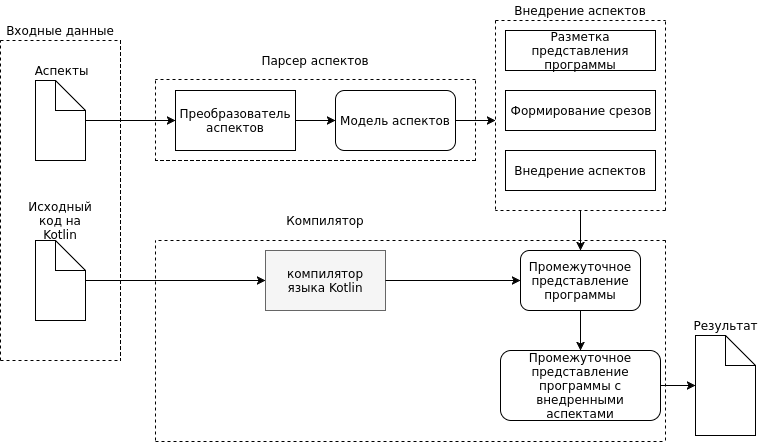
\includegraphics[width=\textwidth]{fig/program_architecture}
\caption{Архитектура программной системы}%
\label{fig:program_architecture}
\end{figure}

Как видно из рисунка~\ref{fig:program_architecture}, система состоит из
следующих частей:
\begin{enumerate}
	\item Первой частью системы являются преобразователи, отвечающие за
		 импортирование исходного кода и описания аспектов и приведения их к
		 виду промежуточного представления.
		 Для создания преобразователя аспектов, необходимо сформировать
		 грамматику описания аспектов.
		 Создание промежуточного представления программы может быть переложено
		 на компилятор языка Kotlin.
	\item Второй частью системы является часть, отвечающая за внедрение аспектов
		в промежуточное представление программы.
		Данная часть состоит из нескольких компонентов: части, отвечающей за
		разметку промежуточного представления, части, отвечающей за формирование
		срезов и части, реализующей внедрение аспектов.
	\item Последней частью системы является часть, отвечающая за компиляцию
		модифицированного промежуточного представления программы в байт-код.
		Данную часть также нет необходимости реализовывать полностью самому, так
		как можно воспользоваться готовыми системами сборки, передав в них
		не исходные коды программы, а модифицированное промежуточное
		представление.
\end{enumerate}

Таким образом, основное внимание стоит уделить модулям, отвечающим за построение
модели аспектов и внедрению аспектов в промежуточное представление программы.
%%%%%%%%%%%%%%%%%%%%%%%%%%%%%%%%%%%%%%%%%%%%%%%%%%%%%%%%%%%%%%%%%%%%%%%%%%%%%%%%
\section{Разработка синтаксиса аспектов}
\label{sec:aspect_syntax_design}
%%%%%%%%%%%%%%%%%%%%%%%%%%%%%%%%%%%%%%%%%%%%%%%%%%%%%%%%%%%%%%%%%%%%%%%%%%%%%%%%
По результатам анализа существующих АОП-расширений можно выделить два основных
способа описания аспектов: создание классов, каждый из которых позволяет
производить вставку кода советов или же использование дополнительного синтаксиса
описания аспектов.
Для разрабатываемого прототипа был выбран второй способ, а именно, создание
отдельного синтаксиса описания аспектов, схожего с описанием классов в языке
Kotlin.

За основу разрабатываемого синтаксиса было решено взять язык описания аспектов,
используемый в фреймворке AspectJ.
Данный выбор был сделан, во-первых, из-за большой популярности данного
АОП-расширения и, во-вторых, из-за удобства и гибкости данного способа описания
аспектов.
%%%%%%%%%%%%%%%%%%%%%%%%%%%%%%%%%%%%%%%%%%%%%%%%%%%%%%%%%%%%%%%%%%%%%%%%%%%%%%%%
\subsubsection{Синтаксис описания аспекта}
\label{ssub:custom_aspect_syntax}
%%%%%%%%%%%%%%%%%%%%%%%%%%%%%%%%%%%%%%%%%%%%%%%%%%%%%%%%%%%%%%%%%%%%%%%%%%%%%%%%
Как и в AspectJ, сквозная функциональность инкапсулируется в сущности,
называемой \textit{аспект}.
Каждый аспект имеет свой уникальный идентификатор и может содержать как описание
советов и срезов, так и переменные и функции, предназначенные для внутреннего
использование.
Описание аспекта, в целом, похоже на описание класса в языке Kotlin: оно
начинается с ключевого слова \textit{aspect}, после чего следует идентификатор
аспекта и, затем, тело аспекта, заключенное в фигурные скобки.
Пример описания аспекта с идентификатором \textit{FooAspect} приведен в листинге
~\ref{lst:custom_aspect_example}.
  \begin{lstlisting}[language=Java, label={lst:custom_aspect_example}, 
  caption={Пример описания аспекта в разрабатываемом прототипе}]
aspect FooAspect  {
  ... Тело аспекта
}
  \end{lstlisting}
%%%%%%%%%%%%%%%%%%%%%%%%%%%%%%%%%%%%%%%%%%%%%%%%%%%%%%%%%%%%%%%%%%%%%%%%%%%%%%%%
\subsubsection{Синтаксис описания срезов}
\label{ssub:custom_pointcut_syntax}
%%%%%%%%%%%%%%%%%%%%%%%%%%%%%%%%%%%%%%%%%%%%%%%%%%%%%%%%%%%%%%%%%%%%%%%%%%%%%%%%

%%%%%%%%%%%%%%%%%%%%%%%%%%%%%%%%%%%%%%%%%%%%%%%%%%%%%%%%%%%%%%%%%%%%%%%%%%%%%%%%
